\section{Exploratory Data Analysis}

\subsection{Tweet Length Statistics}

Table~\ref{tab:eda_length} summarises text length statistics measured at both the character and word levels for the training and official test splits.

\begin{table}[H]
    \centering
    \caption{Tweet length statistics for the training and test splits.}
    \label{tab:eda_length}
    \begin{tabularx}{\textwidth}{l r r r r r r}
        \toprule
        \textbf{Split} & \textbf{Mean chars} & \textbf{Std chars} & \textbf{Max chars} & \textbf{Mean words} & \textbf{Std words} & \textbf{Max words} \\
        \midrule
        Train & 204.20 & 83.48 & 683 & 30.50 & 12.63 & 112 \\
        Test  & 213.44 & 83.55 & 684 & 32.91 & 13.14 & 110 \\
        \bottomrule
    \end{tabularx}
\end{table}

The test split has slightly longer tweets on average (+9.24 characters, +2.41 words). This is consistent with the temporal shift hypothesis: later-stage pandemic discourse may have included longer, more elaborate commentary. Figure~\ref{fig:word_count} shows the word-count distribution for both splits.

\begin{figure}[H]
    \centering
    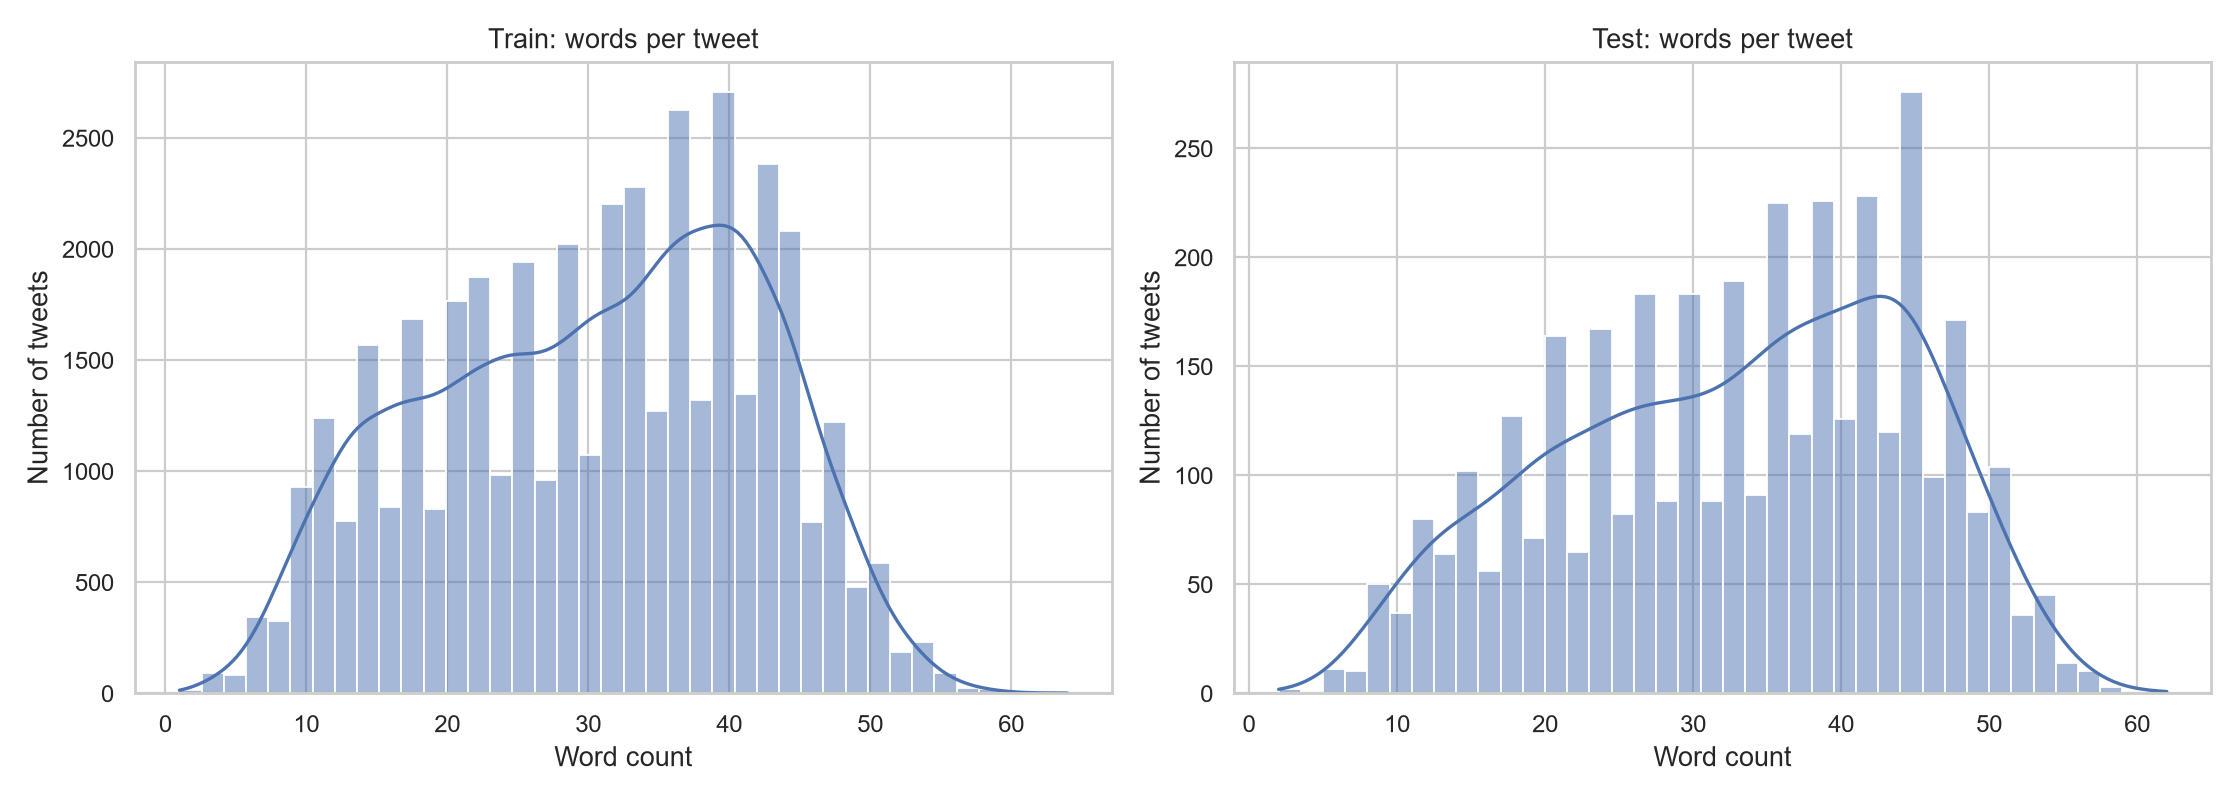
\includegraphics[width=0.80\textwidth]{../../Assignment2/corona_eda/word_count_distribution.png}
    \caption{Word count distribution for the training (blue) and test (orange) splits.}
    \label{fig:word_count}
\end{figure}

\subsection{Temporal Distribution}

A key characteristic of this dataset is its \textbf{inverted temporal ordering}: the official test split was collected \textit{before} the training split.

\begin{itemize}
    \item \textbf{Training split date range:} March 16 -- April 14, 2020
    \item \textbf{Test split date range:} March 2 -- March 16, 2020
\end{itemize}

This means models are trained on later data and evaluated on earlier data, reversing the standard temporal evaluation setting. As pandemic sentiment evolved rapidly during this period (early fear and shock in March vs.\ more nuanced discourse in April), models may face a systematic distributional shift that reduces test performance relative to validation performance. Figures~\ref{fig:train_daily} and~\ref{fig:test_daily} show the daily tweet counts for each split.

\begin{figure}[H]
    \centering
    \begin{minipage}{0.48\textwidth}
        \centering
        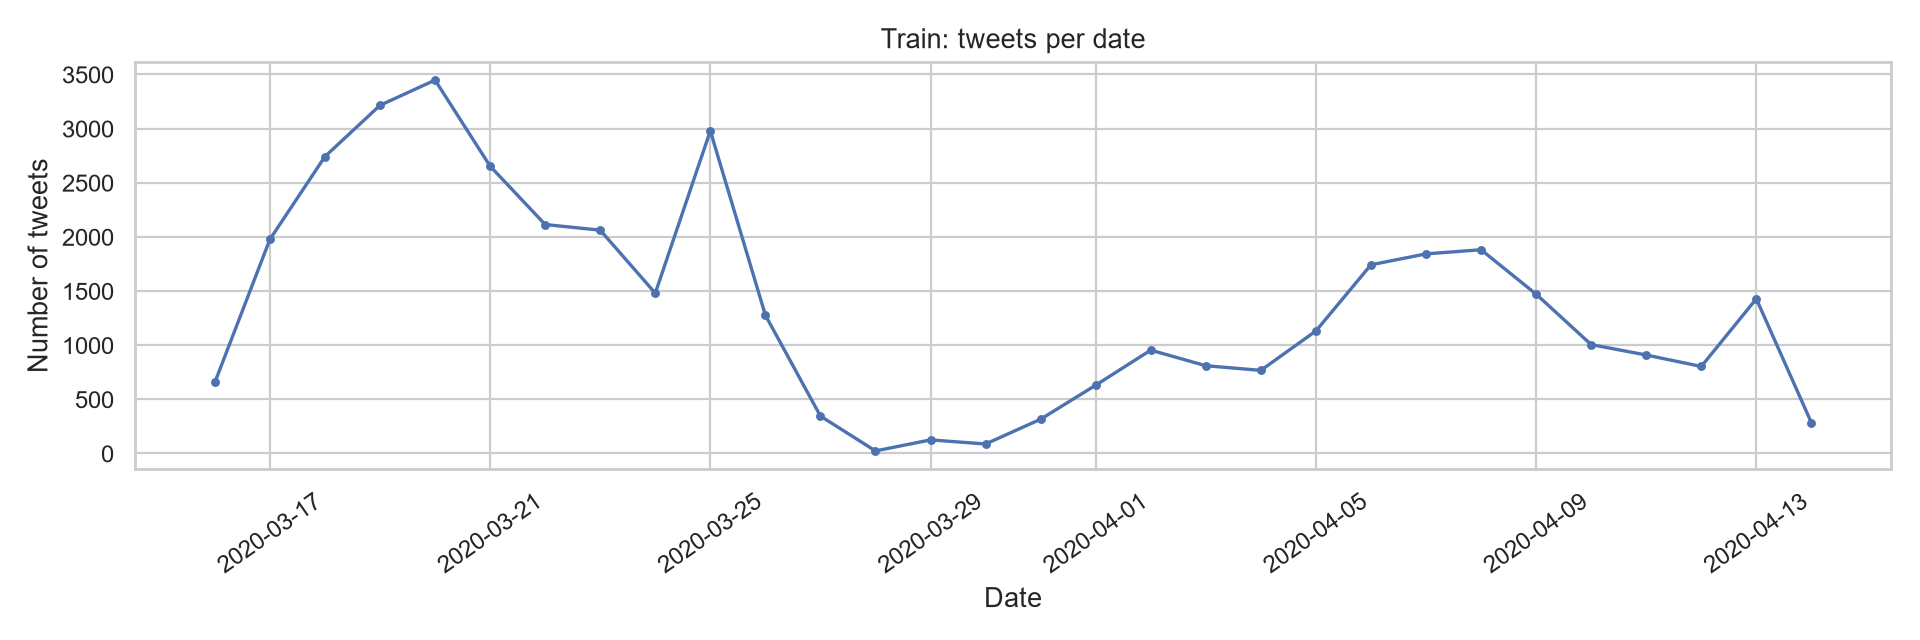
\includegraphics[width=\textwidth]{../../Assignment2/corona_eda/train_daily_counts.png}
        \caption{Daily tweet counts in the training split (March 16 -- April 14, 2020).}
        \label{fig:train_daily}
    \end{minipage}
    \hfill
    \begin{minipage}{0.48\textwidth}
        \centering
        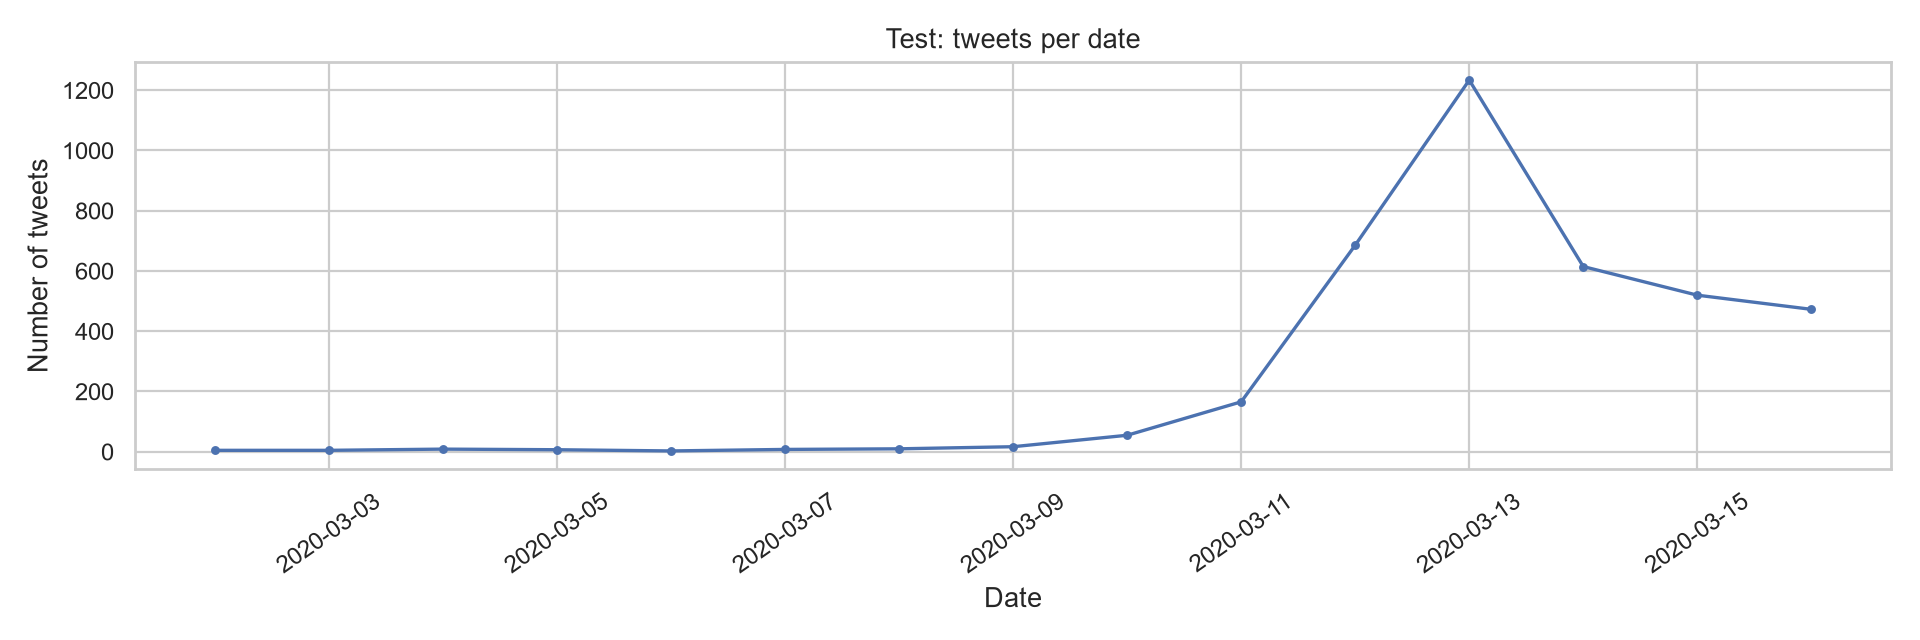
\includegraphics[width=\textwidth]{../../Assignment2/corona_eda/test_daily_counts.png}
        \caption{Daily tweet counts in the test split (March 2 -- March 16, 2020).}
        \label{fig:test_daily}
    \end{minipage}
\end{figure}

\subsection{Representative Samples per Class}

Table~\ref{tab:representative_samples} presents illustrative tweet examples from each sentiment class, chosen to highlight the annotation challenges and boundary ambiguity between adjacent classes.

\begin{table}[H]
    \centering
    \caption{Representative tweet samples by sentiment class.}
    \label{tab:representative_samples}
    \begin{tabularx}{\textwidth}{l X}
        \toprule
        \textbf{Class} & \textbf{Sample Tweet} \\
        \midrule
        Extremely Negative
            & \textit{``This is an absolute catastrophe. Hospitals are overwhelmed, people are dying alone, and the government is doing NOTHING. \#COVID19''}\\
        \addlinespace
        Negative
            & \textit{``Worried about my elderly parents during this pandemic. Trying to keep them safe but it's so stressful. \#coronavirus''}\\
        \addlinespace
        Neutral
            & \textit{``The WHO has released new guidelines on hand washing and social distancing to prevent the spread of COVID-19. \#health''}\\
        \addlinespace
        Positive
            & \textit{``So heartwarming to see neighbours helping each other during \#lockdown. Dropping off groceries for the vulnerable.''}\\
        \addlinespace
        Extremely Positive
            & \textit{``AMAZING news!! Scientists report promising results from early vaccine trials! Hope is on the horizon! \#COVID19vaccine \#science''}\\
        \bottomrule
    \end{tabularx}
\end{table}

\subsection{Key EDA Findings}

\begin{enumerate}
    \item Tweets are uniformly long (mean $\approx$ 30 words), substantially longer than many standard sentiment datasets such as SST-2.
    \item The test split is marginally but consistently longer than the training split, corroborating the temporal shift.
    \item Deduplication is not critical (only 15 duplicates out of 41,157 training rows; 1 cross-split overlap).
    \item Adjacent class pairs (\textit{Negative}/\textit{Extremely Negative}; \textit{Positive}/\textit{Extremely Positive}) share similar vocabulary and are likely the dominant source of classification errors.
\end{enumerate}
